% Number 391
% CAPMA Algebra Units
% Meteor chunk slowdown; algebraic version
% JG

% Watermark
\AddToShipoutPicture*{\BackgroundPic}

\addtocounter {ProbNum} {1}

%\begin{floatingfigure}[r]{.15\textwidth}
%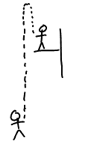
\includegraphics[scale=.8]{/Users/jgates/desktop/latex/pics/tokentoss.png}
%\end{floatingfigure}
 
{\bf \Large{\arabic{ProbNum}}} A rock fragment is traveling ${640~\tfrac{m}{s}}$  when it is knocked off of a falling meteor. It has slowed to ${590~\tfrac{m}{s}}$  after .6 seconds.  Assume a constant acceleration. 

\bigskip
How far will it have gone after 2 seconds? Use algebraic problem-solving.

%\begin{center}
%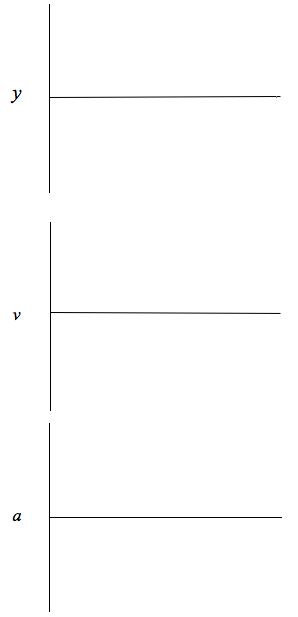
\includegraphics[scale=.85]{/Users/jgates/desktop/latex/pics/blankyvagraphstack.png}
%\end{center}


\vfill
\newpage
